\documentclass[../diploma.tex]{subfiles}
 
\begin{document}

В сообществе специалистов в области машинного обучения последние годы проселживается пока ещё незаутхающий интерес к нейронным сетям. 
На мнгоих побуличных выступлениях любят говорит о том, что дешёные GPU дали второе дыхание нейронным сетям. 
Вы также можете услышать об открытых соревнованиях, на которых решения, основанные на глубинном обучении, добились такой точности, что отнесли считавшуюся ранее открытой проблему в разряд решённых.
Одним из таких знаменитых примеров стало закрытие проекта Asirra\cite{elson2007asirra} в результате контеста на Kaggle\cite{kaggle:dogcats}. 

В этой работе мы не нацеливались на какие-то выдающиеся результаты в плане точности.
Дело в том, что самые последние \hyperref[sec:existing_solutions]{исследования} \autoref{sec:existing_solutions} в сфере генерации голоса публикуются исследовательскими коммандами крупных корпорации с большими вычислительными ресурсами. 

Публикация \cite{article:van2016wavenet}, на результатах котороой основана данная работа  не исключение.
Мы не собирались соревноваться в качестве генерации с существующими решениями. Нам захотелось развить идею придачи дополнительных характеристик генерируемому голосу. Такие характеристики можно придумать самые разные: от простого мужской/женский голос до имитации речи конкретного человека.

% Мы, в свою очередь попытаемся реализовать необычное применение к старым методам. 
% Причём наши исследования воспроизводимы даже в домашних усслових для более или менее пт риличной конфигурации ПК.

% Хотелось бы внести свой вклад в 
Инструментарий для таких целей имеется WaveNet \cite{article:van2016wavenet}, однако только с точки зрения архитектуры и совсем без описания дополнительных признаков. Мы посчитали, что более подробное исследование этого ворпоса и получение практических результатов было бы достойным вкладом в исследовательское сообщество.

\subsection{Применения}

Сразу видится большое количество практических применений такого исследования от персонализорованного голоса в навигаторе до эмуляции голосов знаменитосей. Конечно разработка такой полноценной произведоственной системы достаточно сложная задача и выходит далеко за рамки данной работы. Однако мы должны понимать, как должен выглядеть внешний интерфейс взаимодействия с моделью, чтобы последняя была полезна на практите. 

Высокоуровневый макет предполагаемой системы изображен на рисунке \ref{fig:speech_system}.

\begin{figure}[h!]
  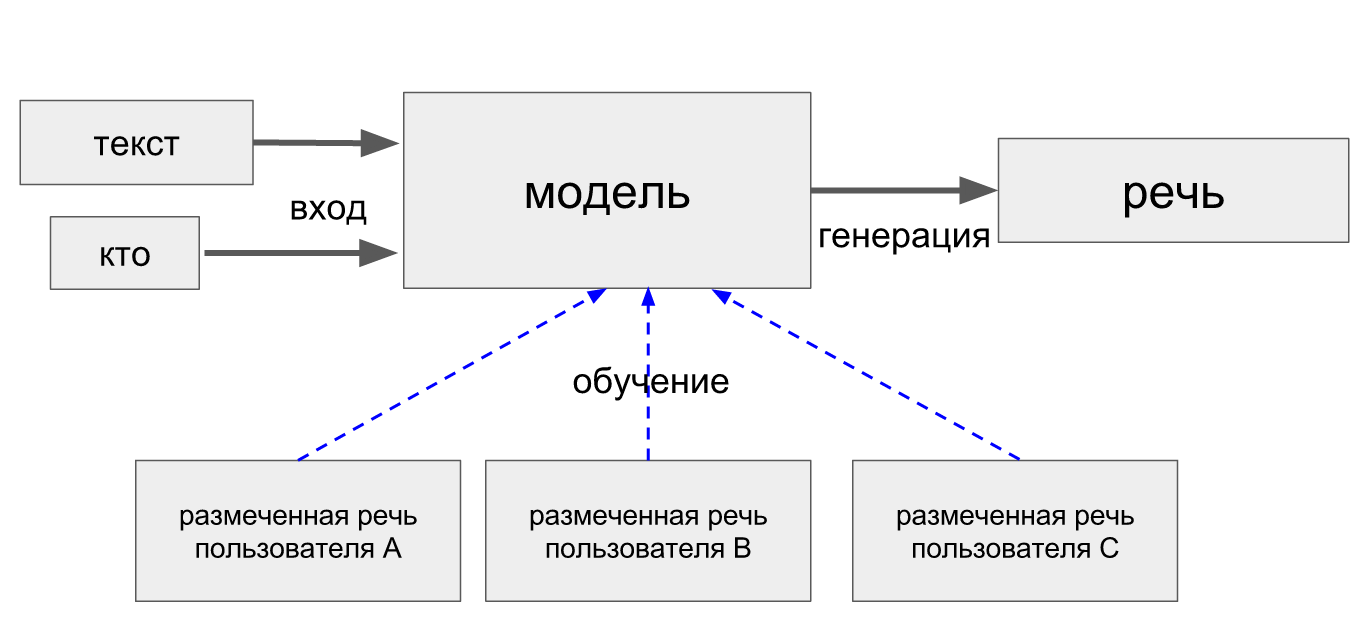
\includegraphics[scale=0.36]{img/scheme}
  \caption{Система генерации речи}
  \label{fig:speech_system}
\end{figure}

\pagebreak
\end{document}

Хоть и представления о такой модели достаточно утопично, опишем, как бы мы хотели, чтобы она работала в иделе.
Изображенная система должна быть преобучена на некоторой базе пользователей, для каждого из которых было предоставлено достаточное количество записей голоса вместе с выровненным вдоль него произнесенным текстом. 

На вход должен подаваться текст, выровненный с некоторыми признаками, которые мы назовём локальные условия и какой-то общей хараткеристкой, например, описывающей, чей голос мы хотим сгенерировать. Такую характеристику назовём глобальным условием. 

На выходе мы ожидаем получить речь с нужными нам особенностями.